\documentclass[11pt]{article}
\usepackage{acl04}
\usepackage{times}
\usepackage{latexsym}
\usepackage{url,alltt,epsfig,boxedminipage}

% hyphenation control
\pretolerance 250
\tolerance 500
\hyphenpenalty 200
\exhyphenpenalty 100
\doublehyphendemerits 7500
\finalhyphendemerits 7500
\brokenpenalty 10000
\lefthyphenmin 3
\righthyphenmin 3
\widowpenalty 10000
\clubpenalty 10000
\displaywidowpenalty 10000
\looseness 1

\def\UrlFont{\tt\small}
\def\object#1{\texttt{\small #1}}

\title{NLTK: The Natural Language Toolkit}

\author{
  Steven Bird \\
  Department of Computer Science \\
  \indent and Software Engineering \\
  University of Melbourne \\
  Victoria 3010, Australia \\  
  {\tt sb@csse.unimelb.edu.au}
\And
  Edward Loper\\
  Department of Computer \\
  \indent and Information Science \\
  University of Pennsylvania\\
  Philadelphia PA 19104-6389, USA\\
  {\tt edloper@gradient.cis.upenn.edu}
}

\date{}

\newenvironment{sv}{\scriptsize\begin{alltt}}{\end{alltt}\normalsize}

\begin{document}

\maketitle

\begin{abstract}\small
  The Natural Language Toolkit is a suite of program modules, data
  sets, tutorials and exercises, covering symbolic and statistical
  natural language processing.  NLTK is written in Python and
  distributed under the GPL open source license.  Over the past three
  years, NLTK has become popular in teaching and research.  We
  describe the toolkit and report on its current state of development.
\end{abstract}

%========================= Introduction =========================
\section{Introduction}

The Natural Language Toolkit (NLTK) was developed in conjunction with
a computational linguistics course at the University of Pennsylvania
in 2001 \cite{LoperBird02}.  It was designed with three pedagogical
applications in mind: assignments, demonstrations, and projects.

\textbf{Assignments.}
NLTK supports assignments of varying difficulty
and scope.  In the simplest assignments, students experiment with
existing components to perform a wide variety of NLP tasks.  As students
become more familiar with the toolkit, they can be asked to modify
existing components, or to create complete systems out of existing
components.

\textbf{Demonstrations.}
NLTK's interactive graphical demonstrations have proven to be very
useful for students learning NLP concepts.
The demonstrations give a step-by-step execution of important
algorithms, displaying the current state of key data structures.
A screenshot of the chart parsing demonstration is shown in Figure~\ref{fig:chart}.

\textbf{Projects.}  NLTK provides students with a flexible framework
for advanced projects.  Typical projects might involve implementing a
new algorithm, developing a new component, or adding support for a new
task.

We chose Python because it has a shallow learning curve, its syntax
and semantics are transparent, and it has good string-handling
functionality.  As an interpreted language, Python facilitates
interactive exploration.  As an object-oriented language, data and
methods can be encapsulated easily.  Python comes with an extensive
standard library, including tools for graphical programming and
intensive numerical processing.  And the recently added generator
syntax makes it easy to create interactive implementations of
algorithms \cite{Loper04,Rossum03intro,Rossum03ref}.

\begin{figure}[bth]
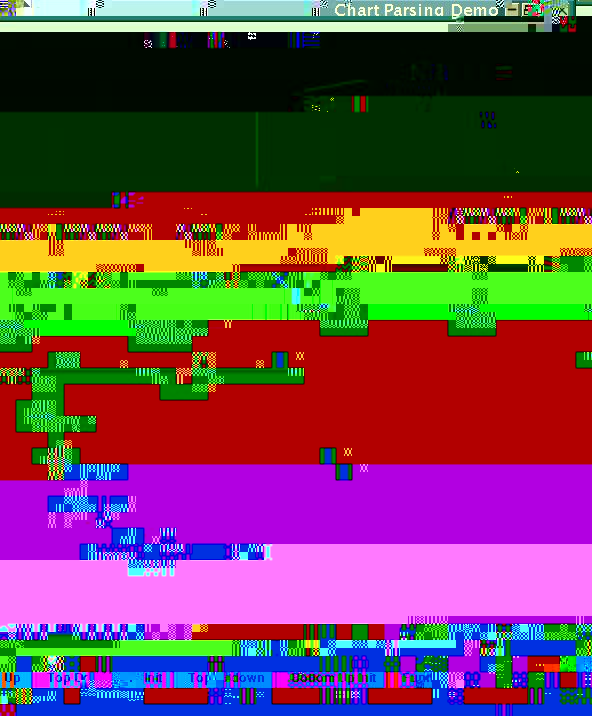
\epsfig{file=../pycon2004/chart.eps, width=\linewidth}
\caption{Interactive Chart Parsing Demonstration}
\label{fig:chart}
\end{figure}

\section{Design}

NLTK is implemented as a large collection of minimally interdependent
modules, organized into a shallow hierarchy.  A set of core
modules defines basic data types that are used throughout the toolkit.
The remaining modules are \emph{task modules}, each devoted to an
individual natural language processing task.  For example, the
\object{nltk.parser} module encompasses to the task of
\emph{parsing}, or deriving the syntactic structure of a sentence; and
the \object{nltk.tokenizer} module is devoted to the task of
\emph{tokenizing}, or dividing a text into its constituent parts.

\subsection{Tokens and other core data types}

To maximize interoperability between modules, we use a
single class to encode information about natural language texts -- the
\object{Token} class.  Each \object{Token} instance represents a
single unit of text, such as a word, sentence, or document; and is
defined by a (partial) mapping from property names to values.  For
example, the \object{TEXT} property is used to encode a token's text
content:\footnote{Some code samples are specific to NLTK
  version 1.4.}

\begin{alltt}\small
\textbf{>>> from nltk.token import *}
\textbf{>>> Token(TEXT="Hello World!")}
<Hello World!>
\end{alltt}
%
The \object{TAG} property is used to encode a token's part-of-speech
tag:

\begin{alltt}\small
\textbf{>>> Token(TEXT="python", TAG="NN")}
<python/NN>
\end{alltt}
%
The \object{SUBTOKENS} property is used to store a tokenized text:

\begin{alltt}\small
\textbf{>>> from nltk.tokenizer import *}
\textbf{>>> token = Token(TEXT="Hello World!")}
\textbf{>>> WhitespaceTokenizer().tokenize(token)}
\textbf{>>> print token['SUBTOKENS'])}
[<Hello>, <World!>]
\end{alltt}
%
In a similar fashion, other language processing tasks such as
word-sense disambiguation, chunking and parsing all add properties to
the \object{Token} data structure.

In general, language processing tasks are formulated as
annotations and transformations involving \object{Tokens}.  In
particular, each processing task takes a token, and extends it to
include new information.  Typically, these modifications are
\emph{monotonic}; in other words, new information is added but
existing information is not deleted or modified.  Thus, tokens serve
as a \emph{blackboard}, where information about a piece of text is
collated.  This architecture contrasts with the more typical
\emph{pipeline} architecture, where each processing task's output
discards its input information.  We chose the ``blackboard'' approach
over the ``pipeline'' approach because it allows more flexibility when
combining tasks into a single system.

In addition to the \object{Token} class and its derivatives, NLTK
defines a variety of other data types.  For instance, the
\object{nltk.probability} module defines classes for
probability distributions and statistical smoothing techniques; and
the \object{cfg} module defines classes for encoding context free
grammars and probabilistic context free grammars.

\subsection{The corpus module}

\begin{table*}
\small\noindent
\begin{boxedminipage}{\linewidth}
\begin{tabular}{llll}
\textbf{Corpus} &
\textbf{Contents and Wordcount} &
\textbf{Example Application} \\

20 Newsgroups (selection) &
3 newsgroups, 4000 posts, 780kw &
text classification \\

Brown Corpus &
15 genres, 1.15Mw, tagged &
training and testing taggers, text classification \\

CoNLL 2000 Chunking Data &
270kw, tagged and chunked &
training and testing chunk parsers \\

Project Gutenberg (selection) &
14 texts, 1.7Mw &
text classification, language modelling \\

NIST 1999 IEER (selection) &
63kw, named-entity markup &
training and testing named-entity recognizers \\

Levin Verb Index &
3k verbs with Levin classes &
parser development \\

Names Corpus &
8k male and female names &
text classification \\

PP Attachment Corpus &
28k prepositional phrases, tagged &
parser development \\

Roget's Thesaurus &
200kw, formatted text &
word-sense disambiguation \\

SEMCOR &
880kw, POS and sense tagged &
word-sense disambiguation \\

SENSEVAL 2 Corpus &
600kw, POS and sense tagged &
word-sense disambiguation \\

Stopwords Corpus &
2,400 stopwords for 11 lgs &
text retrieval \\

Penn Treebank (sample) &
40kw, tagged and parsed &
parser development \\

Wordnet 1.7 &
180kw in a semantic network &
word-sense disambiguation, NL understanding \\

Wordlist Corpus &
960kw and 20k affixes for 8 lgs &
spell checking
 \\
\end{tabular}
\caption{Corpora and Corpus Samples Distributed with NLTK}\label{tab:data}
\end{boxedminipage}
\end{table*}

Many language processing tasks must be developed and tested using
annotated data sets, or corpora.  Several such corpora are distributed
with NLTK, as listed in Table~\ref{tab:data}.  The NLTK
\object{corpus} module defines classes for reading and processing
many of these corpora.  The following code fragment illustrates
how the Brown Corpus is accessed.

\begin{alltt}\small
\textbf{>>> from nltk.corpus import brown}
\textbf{>>> brown.groups()}
['skill and hobbies', 'popular lore', 
'humor', 'fiction: mystery', ...]
\textbf{>>> brown.items('humor')}
('cr01', 'cr02', 'cr03', 'cr04', 'cr05',
'cr06', 'cr07', 'cr08', 'cr09')
\textbf{>>> brown.tokenize('cr01')}
<[<It/pps>, <was/bedz>, <among/in>,
<these/dts>, <that/cs>, <Hinkle/np>,
<identified/vbd>, <a/at>, ...]>
\end{alltt}
%
A selection of 5\% of the Penn Treebank corpus is included with
NLTK, and it is accessed as follows:

\begin{alltt}\small
\textbf{>>> from nltk.corpus import treebank}
\textbf{>>> treebank.groups()}
('raw', 'tagged', 'parsed', 'merged')
\textbf{>>> treebank.items('parsed')}
['wsj_0001.prd', 'wsj_0002.prd', ...]
\textbf{>>> item = 'parsed/wsj_0001.prd'}
\textbf{>>> sentences = treebank.tokenize(item)}
\textbf{>>> for sent in sentences['SUBTOKENS']:}
\textbf{...     print sent.pp()} \emph{# pretty-print}
(S:
  (NP-SBJ:
    (NP: <Pierre> <Vinken>)
    ...
\end{alltt}
%

\subsection{Processing modules}

Each language processing algorithm is implemented as a class.  For
example, the \object{ChartParser} and
\object{Recursive\-Descent\-Parser} classes each define a single
algorithm for parsing a text.  We implement language processing
algorithms using classes instead of functions for three reasons.
First, all algorithm-specific options can be passed to the
constructor, allowing a consistent interface for applying the
algorithms.  Second, a number of algorithms need to have their state
initialized before they can be used.  For example, the
\object{NthOrderTagger} class must be initialized by training on a
tagged corpus before it can be used.  Third, subclassing can be used
to create specialized versions of a given algorithm.

Each processing module defines an \emph{interface} for its task.
Interface classes are distinguished by naming them with a trailing
capital ``\object{I},'' such as \object{ParserI}.
Each interface defines a single \emph{action method}, which actually
performs the task defined by the interface.  For example, the
\object{ParserI} interface defines the \object{parse} method; and the
\object{Tokenizer} interface defines the \object{tokenize} method.
When appropriate, an interface defines \emph{extended action
  methods}, which provide variations on the basic action method.  For
example, the \object{ParserI} interface defines the \object{parse\_n}
method, which finds at most $n$ parses for a given sentence; and
the \object{TokenizerI} interface defines the \object{xtokenize}
method, which outputs an iterator over subtokens instead of a list of
subtokens.

\subsection{Documentation}

Three different types of documentation are available.  Tutorials
explain how to use the toolkit, with detailed worked examples.  The
API documentation describes every module, interface, class, method,
function, and variable in the toolkit.  Technical reports explain and
justify the toolkit's design and implementation.  All are available
from \url{http://nltk.sf.net/docs.html}.

\section{Installing NLTK}

NLTK is available from \url{nltk.sf.net}, and is packaged for
easy installation under Unix, Mac OS X and Windows.  The full
distribution consists of four packages: the Python source code
(\object{nltk}); the corpora (\object{nltk-data}); the documentation
(\object{nltk-docs}); and third-party contributions
(\object{nltk-contrib}).  Before installing NLTK, it is necessary to
install Python version 2.3 or later, available from
\url{www.python.org}.  Full installation instructions and a quick
start guide are available from the NLTK homepage.

As soon as NLTK is installed, users can run the demonstrations.  On
Windows, the demonstrations can be run by double-clicking on their
Python source files.  Alternatively, from the Python interpreter, this
can be done as follows:

\begin{alltt} \small
\textbf{>>> import nltk.draw.rdparser}
\textbf{>>> nltk.draw.rdparser.demo()}
\textbf{>>> nltk.draw.srparser.demo()}
\textbf{>>> nltk.draw.chart.demo()}
\end{alltt}

\section{Using and contributing to NLTK}

NLTK has used at the University of Pennsylvania since 2001, and has
subsequently been adopted by several NLP courses at other
universities, including those listed in Table~\ref{tab:courses}.

Third party contributions to NLTK include: Brill tagger (Maloof),
hidden Markov model tagger (Cohn), GPSG-style feature-based grammar
and parser (Speer, Berwick), Kimmo finite-state morphological analyzer
(de Marcken, Yankama, Berwick) and decision list and decision tree
classifiers (Cohn).

NLTK is an open source project, and we welcome any contributions.
There are several ways to contribute: users can report bugs, suggest
features, or contribute patches on Sourceforge; users can participate
in discussions on the \textit{NLTK-Devel} mailing
list\footnote{\url{http://lists.sourceforge.net/lists/listinfo/nltk-devel}}
or in the NLTK public
forums; and users can submit their own NLTK-based projects for
inclusion in the nltk\_contrib directory.  New code modules that are
relevant, substantial, original and well-documented will be considered
for inclusion in NLTK proper.  Potential contributors should note that
all source code is distributed under the GNU General Public License,
and all documentation is distributed under a Creative Commons
non-commercial license.  Thus they can be confident that their
work will remain freely available to all.  Further information about
contributing to NLTK is available at \url{http://nltk.sf.net/contrib.html}.

\begin{table}[bt]
\small\noindent
\begin{boxedminipage}{\linewidth}
\begin{tabular}{l}
University of Pennsylvania, USA \\
\hspace{2ex}
\textit{Introduction to Computational Linguistics} \\[.5ex]

University of Melbourne, Australia \\
\hspace{2ex}
\textit{Human Language Technology} \\[.5ex]

University of Pittsburgh, USA \\
\hspace{2ex}
\textit{Artificial Intelligence Application Development} \\[.5ex]

Simon Fraser University, Canada \\
\hspace{2ex}
\textit{Computational Linguistics} \\[.5ex]

Macquarie University, Australia \\
\hspace{2ex}
\textit{Intelligent Text Processing} \\[.5ex]

University of Edinburgh, UK \\
\hspace{2ex}
\textit{Introduction to Computational Linguistics} \\[.5ex]

National Autonomous University of Mexico, Mexico \\
\hspace{2ex}
\textit{Introduction to Natural Language Processing in Python} \\[.5ex]

University of Magdeburg, Germany \\
\hspace{2ex}
\textit{Natural Language Systems} \\[.5ex]

Massachusetts Institute of Technology, USA \\
\hspace{2ex}
\textit{Natural Language Processing} \\[.5ex]

University of Colorado, USA \\
\hspace{2ex}
\textit{Natural Language Processing} \\[.5ex]

University of Amsterdam, Netherlands \\
\hspace{2ex}
\textit{Language Processing and Information Access} \\[.5ex]

Graz University of Technology, Austria \\
\hspace{2ex}
\textit{Information Search and Retrieval} \\[.5ex]

\end{tabular}
\caption{University Courses using NLTK}\label{tab:courses}
\end{boxedminipage}
\end{table}

\section{Conclusion}

NLTK is a broad-coverage toolkit that provides a simple, extensible,
uniform framework for assignments, demonstrations and projects.  It is
thoroughly documented, easy to learn, and simple to use.  Readers who
would like to receive occasional announcements about NLTK are
encouraged to sign up for the low-volume, moderated mailing list
\textit{NLTK-Announce}\footnote{\url{http://lists.sourceforge.net/lists/listinfo/nltk-announce}}.

\section{Acknowledgements}

We are indebted to our students for feedback on the toolkit, and to
many contributors listed on the NLTK website.

\bibliographystyle{acl}
\bibliography{nltk}

\end{document}

